\documentclass{ximera}

\title{Derivative Rules Part 2 Activity Solution Guide}
\author{MATH 425: Calculus I}

\begin{document}
\begin{abstract}
    Working with the peers in your group, solve the following problems. Make sure to show and justify all your work. Make sure everyone in the group understands the solution and participates. Be prepared to report your answers to the whole class. 
\end{abstract}
\maketitle

\begin{exercise}
    Use the table to answer the following questions.\\  
    \begin{tabular}{c|c|c|c|c}
        x  & $f(x)$ & $g(x)$ & $f'(x)$ & $g'(x)$   \\ \hline
        -1  & $\pi$ & 0 & -1 & 3\\ \hline
        0 & $-\frac12$ & -1 & 0 & 4\\ \hline
        2 & -2 & 7 & 3 & $-\frac{\pi}{4}$ \\ \hline
        3 & 1 & e & $\frac23$ & 0\\%\hline   
    \end{tabular}
    \begin{enumerate}
       \item $\frac{f}{g}(-1)$ \textcolor{blue}{ undefined}
        \item $\frac{g}{f}(0)$ \textcolor{blue}{ $=2$}
        \item $(fg)(2)$ \textcolor{blue}{ $=-14$}
        \item $(3f-2g)(0)$ \textcolor{blue}{ $=\frac12$}
        \item $f(g(-1))$ \textcolor{blue}{ $=-\frac12$}
        \item $\frac{d}{dx} (f+g)(x)$ at $x=3$ \textcolor{blue}{ $\frac23$}
        \item $\frac{d}{dx} (3f+4g)(x)$ at $x=2$ \textcolor{blue}{ $9-\pi$}
        \item $\frac{d}{dx} x^2+f(x)$ at $x=0$ \textcolor{blue}{ $0-\frac12=-\frac12$}
        \item $\frac{d}{dx} \big(\frac{f}{g}(x)\big)$ at $x=3$ \textcolor{blue}{ $\frac{0-\frac{2}{3}e}{e^2}=-\frac{2}{3e}$}
        \item $\frac{d}{dx} (3f(g(x)))$ at $x=-1$ \textcolor{blue}{ $0$}
        \item $\frac{d}{dx} x^2f(x)$ at $x=3$ \textcolor{blue}{ $6+6=12$}
    \end{enumerate}
\end{exercise}

\begin{exercise}
    Use the graph to find the following derivatives.
    \begin{image}
    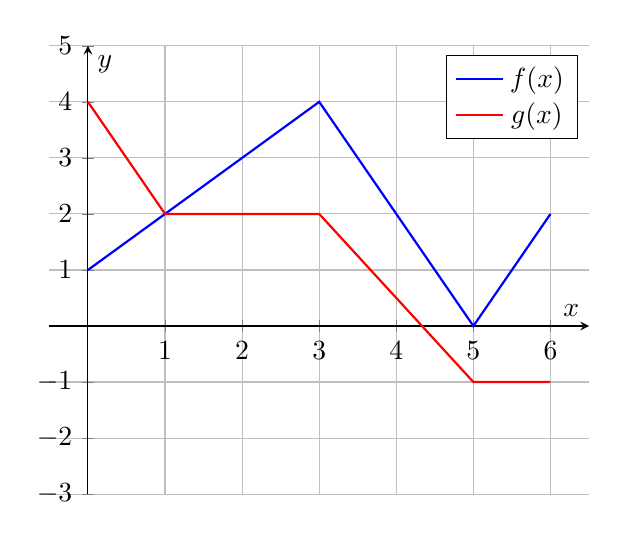
\begin{tikzpicture}[scale=1]
        \begin{axis}[
            xlabel=$x$,
            ylabel=$y$,
            grid=major,
            axis lines=middle,
            xmin=-0.5, xmax=6.5,
            ymin=-3, ymax=5,
            xtick={0,1,2,3,4,5,6},
            ytick={-3,-2,-1,0,1,2,3,4,5}
        ]
        
        % Function f(x): piecewise linear
        \addplot[blue, thick] coordinates {(0,1) (3,4) (5,0) (6,2)};
        \addlegendentry{$f(x)$}
        
        % Function g(x): piecewise linear
        \addplot[red, thick] coordinates {(0,4) (1,2) (3,2) (5,-1) (6,-1)};
        \addlegendentry{$g(x)$}
        
        \end{axis}
    \end{tikzpicture}
\end{image}
    \begin{enumerate}
        \item $f'(1)$ \textcolor{blue}{$=1$}
       \item $g'(5)$ \textcolor{blue}{undefined (corner)}
        \item $fg'(2)$ \textcolor{blue}{$=f(2)g'(2)+g(2)f'(2)=3(0)+2(1)=2$}
        \item $\frac{f}{g}'(4)$ \textcolor{blue}{$\frac{g(4)f'(4)-f(4)g'(4)}{(g(4))^2}=\frac{0.5(-2)-(2)(-1.5)}{(.5)^2}=\frac{2}{.25}=8$}
        \item $(f+g)'(2)$ \textcolor{blue}{$=f'(2)+g'(2)=1+0=1$}
    \end{enumerate}
\end{exercise}

\begin{exercise}
    Calculate the derivative for the following functions using rules from class.  Before attempting the derivative, choose a rule (or rules) and justify to yourself why you are using this rule. 
    \begin{enumerate}
        \item $f(x)=x^{\frac23}\sqrt{(3x^7-x)}$\\
        \textcolor{blue}{ $f'(x)=(3x^7-\sqrt{x})\frac23x^{-\frac13}+x^{\frac23}(21x^6-\frac{1}{2}x^{-\frac{1}{2}})$}

        \item $g(x)=(2x^4-3x^{-3})x^{-\frac{1}{3}}$\\
        \textcolor{blue}{ $g'(x)=\frac{(\sqrt[3]{x}(8x^3+9x^{-4})-(2x^4-3x^{-3})(\frac{1}{3}x^{-\frac{2}{3}})}{(\sqrt[3]{x})^2}$}

        \item $f(z)=(z^2-3z^{\frac{1}{4}})(z-1)^{-1}$\\
        \textcolor{blue}{ $=\frac{z^2-3z^{\frac{1}{4}}}{z-1};\;\; f'(z)=\frac{(z-1)(2z-\frac{3}{4}z^{-\frac{3}{4}})-(z^2-3z^{\frac{1}{4}})(1)}{(z-1)^2}$}

        \item $h(t)=e^2(3t-2)t^{\frac{3}{4}}$\\
        \textcolor{blue}{ $h'(t)=e^2((3t-2)(\frac34x^{-\frac14})+3t^{\frac34})$}

        \item $g(w)=\frac{w^7-3w^2}{15}$ \\
        \textcolor{blue}{ $g'(w)=\frac{7w^6-6w}{15}$}

        \item $p(x)=\frac{\sqrt{x}(x-2)}{x-3}$   \\
        \textcolor{blue}{ $p'(x)=\frac{(x-3)(\sqrt{x}+(\frac{1}{2}x^{-\frac{1}{2}})(x-2))-\sqrt{x}(x-2)}{(x-3)^2}$}

        \item $f(x)=\frac{1}{(x^2-1)(x^2+x+1)}$\\
        \textcolor{blue}{ $f'(x)=-(x^2+1)^{-1}(x^2+x+1)^{-2}(2x+1)-(x^2+1)^{-2}(2x)(x^2+x+1)^{-1}$}
        
        \item $g(x)=(2x-7)^{-1}(x+5)$\\
        \textcolor{blue}{ $g'(x)=(2x-7)^{-1}(1)-2(2x-7)^{-2}(x+5)$}

        \item $v(t)=\frac{\sqrt{t}-1}{\sqrt{t}+1}$\\
        \textcolor{blue}{ $v'(t)=\frac{(\sqrt{t}+1)(\frac{1}{2}t^{-\frac12})-(\sqrt{t}-1)(\frac12t^{-\frac12})}{(\sqrt{t}+1)^2}$}

        
    \end{enumerate}


\end{exercise}

\begin{exercise}
    Find the equation of the tangent line to the graph of $f(x)=\frac{3x-1}{2x^2-7}$ at $x=2$.\\
    \textcolor{blue}{Slope: $f'(x)=\frac{(2x^2-7)(3)-(3x-1)(4x)}{(2x^2-7)^2}$\\
    $f'(2)=\frac{(2(2)^2-7)(3)-(3(2)-1)(4(2))}{(2(2)^2-7)^2}=\frac{3-40}{1}=-37$\\
    $f(2)=\frac{3(2)-1}{2(2)^2-7}=\frac{5}{1}=5$\\
    Tangent line: $y-5=-37(x-2)$}
\end{exercise}



\end{document}
